\documentclass[border=10pt]{standalone}
\usepackage[svgnames]{xcolor}
\usepackage{amsmath}
\usepackage{pgfplots}
\pgfplotsset{compat=newest}
\usepackage[sfdefault]{FiraSans}
\usepackage{FiraMono}
\renewcommand*\familydefault{\sfdefault}
\begin{document}
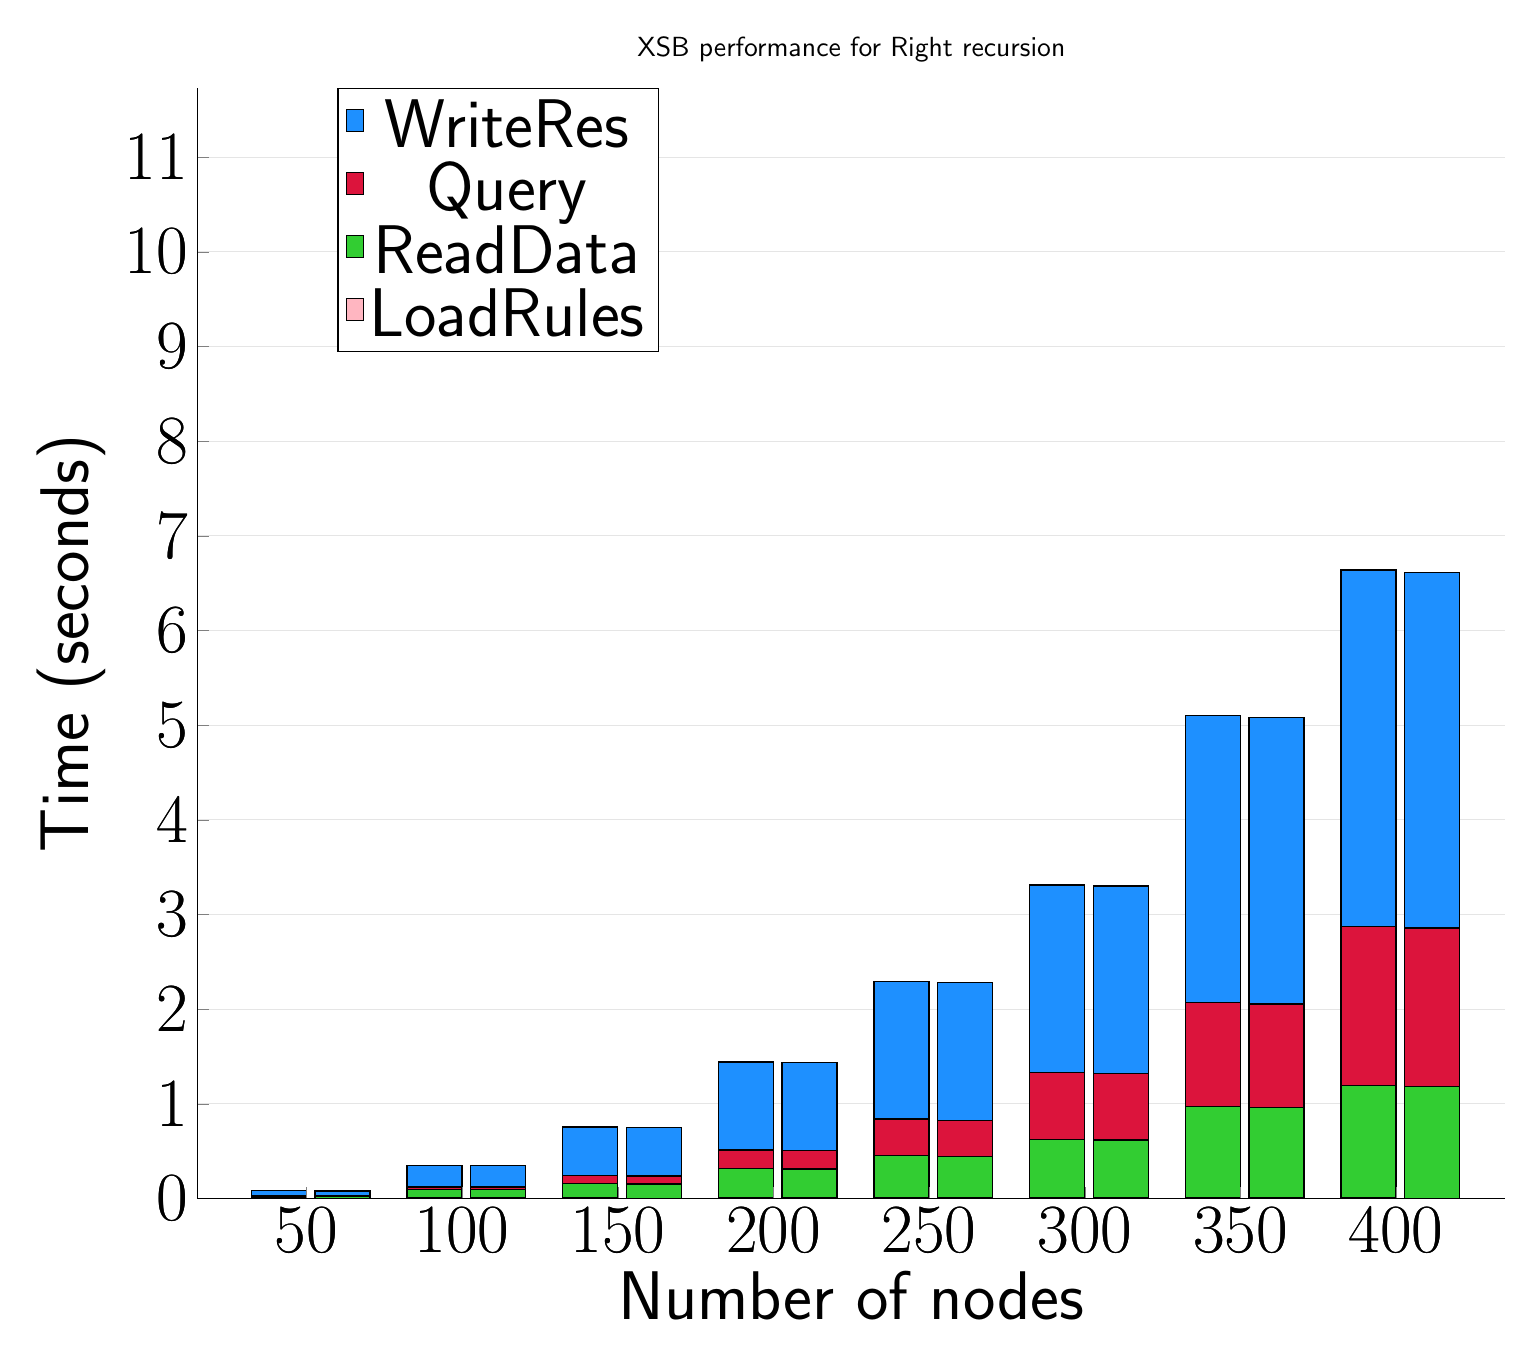
\begin{tikzpicture}
\begin{axis}[
   ybar stacked,
   title={XSB performance for Right recursion},
   bar shift=-10pt,
   width=1.5\textwidth,
   bar width=0.7cm,
   ymajorgrids, tick align=inside,
   major grid style={draw=gray!20},
   xtick=data,
   ymin=0, ymax=11.731267293294271,
   axis x line*=bottom,
   axis y line*=left,
   enlarge x limits=0.1,
   legend style={
       at={(0.23, 1)},
       anchor=north,
       legend columns=1,
       font=\Huge,
   },
   ylabel={Time (seconds)},
   xlabel={Number of nodes},
   label style={font=\Huge},
   tick label style={font=\Huge},
]
\addlegendimage{fill=DodgerBlue, draw=black, line width=0.2pt}
\addlegendentry{WriteRes}
\addlegendimage{fill=Crimson, draw=black, line width=0.2pt}
\addlegendentry{Query}
\addlegendimage{fill=LimeGreen, draw=black, line width=0.2pt}
\addlegendentry{ReadData}
\addlegendimage{fill=LightPink, draw=black, line width=0.2pt}
\addlegendentry{LoadRules}
\addplot +[fill=LightPink, draw=black, line width=0.5pt] coordinates {
    (50, 0.004813989003499347)
    (100, 0.005952358245849609)
    (150, 0.0044376055399576834)
    (200, 0.004722992579142253)
    (250, 0.00487995147705078)
    (300, 0.004476626714070637)
    (350, 0.004726648330688474)
    (400, 0.00440843900044759)
};
\addplot +[fill=LimeGreen, draw=black, line width=0.5pt] coordinates {
    (50, 0.020083347956339533)
    (100, 0.08723735809326173)
    (150, 0.15526342391967765)
    (200, 0.31002656618754065)
    (250, 0.45077697436014796)
    (300, 0.61981471379598)
    (350, 0.966700951258341)
    (400, 1.18921955426534)
};
\addplot +[fill=Crimson, draw=black, line width=0.5pt] coordinates {
    (50, 0.003403027852376303)
    (100, 0.028684933980306)
    (150, 0.08342130978902183)
    (200, 0.19762078921000167)
    (250, 0.3837823073069256)
    (300, 0.7051569620768227)
    (350, 1.10136731465658)
    (400, 1.6783933639526367)
};
\addplot +[fill=DodgerBlue, draw=black, line width=0.5pt] coordinates {
    (50, 0.05371967951456707)
    (100, 0.230585734049479)
    (150, 0.5137483278910319)
    (200, 0.9291958808898917)
    (250, 1.4541974067687977)
    (300, 1.9816961288452173)
    (350, 3.03080042203267)
    (400, 3.7659292221069367)
};
\end{axis}
\begin{axis}[
   ybar stacked,
   bar shift=13pt,
   width=1.5\textwidth,
   bar width=0.7cm,
   ymajorgrids, tick align=inside,
   major grid style={draw=none},
   xtick=data,
   ymin=0, ymax=11.731267293294271,
   axis x line*=none,
   axis y line*=none,
   enlarge x limits=0.1,
   label style={font=\Huge},
   tick label style={font=\Huge},
]
\addplot +[fill=LightPink, draw=black, line width=0.5pt] coordinates {
    (50, 0.0027663333333333338)
    (100, 0.0059529999999999965)
    (150, 0.0033749999999999995)
    (200, 0.004127666666666667)
    (250, 0.00438433333333333)
    (300, 0.00404633333333333)
    (350, 0.0045093333333333365)
    (400, 0.0038996666666666637)
};
\addplot +[fill=LimeGreen, draw=black, line width=0.5pt] coordinates {
    (50, 0.019910666666666667)
    (100, 0.08723233333333334)
    (150, 0.15247733333333333)
    (200, 0.3099403333333333)
    (250, 0.442143)
    (300, 0.6132673333333333)
    (350, 0.9574886666666668)
    (400, 1.178814)
};
\addplot +[fill=Crimson, draw=black, line width=0.5pt] coordinates {
    (50, 0.0032759999999999964)
    (100, 0.028692333333333334)
    (150, 0.08312466666666667)
    (200, 0.19486100000000003)
    (250, 0.380474)
    (300, 0.7018733333333333)
    (350, 1.0950486666666666)
    (400, 1.6752976666666666)
};
\addplot +[fill=DodgerBlue, draw=black, line width=0.5pt] coordinates {
    (50, 0.051947)
    (100, 0.23057000000000002)
    (150, 0.5140876666666666)
    (200, 0.9286819999999999)
    (250, 1.4531189999999998)
    (300, 1.9822016666666666)
    (350, 3.0218043333333333)
    (400, 3.7561436666666665)
};
\end{axis}
\end{tikzpicture}

\end{document}
